\section{Network clustering of simulated networks}\label{sec:network-clustering-of-simulated-networks}

\paragraph{Simulation settings}

For all models we simulate \(M = 9\) networks with
\(\forall m \in \{ 1 \dots M \} , n^m_1 = n^m_2 = 75\) with
\(Q_1 = Q_2 = 3\). For the simulations the proportions are the
following:

\begin{align*}
\bm{\pi}^1 = \left( 0.2, 0.3, 0.5 \right) & &  \bm{\rho}^1 = \left( 0.2, 0.3, 0.5 \right)
\end{align*} and for all \(m = 2,\dots,9\) \begin{align*}
\bm{\pi}^m = \begin{cases}
    \bm{\pi}^1 & \text{for } iid\text{-}colBiSBM \\
    \sigma^1_m(\bm{\pi}^1) & \text{for } \pi\text{-}colBiSBM \text{ and } \pi\rho\text{-}colBiSBM
\end{cases}\\
\bm{\rho}^m =
\begin{cases}
    \bm{\rho}^1 & \text{for } iid\text{-}colBiSBM \\
    \sigma^2_m(\bm{\rho}^1) & \text{for } \rho\text{-}colBiSBM \text{ and } \pi\rho\text{-}colBiSBM
\end{cases}
\end{align*} where \(\sigma^1_m\) and \(\sigma^2_m\) are permutations of
\{1, 2, 3\} proper to network \(m\) and
\(\sigma^1 (\pi)= {(\pi_{\sigma^1 (i)})}_{i=\{1,\dots,3\}}\) and
\(\sigma^2 (\rho)= {(\rho_{\sigma^2 (i)})}_{i=\{1,\dots,3\}}\). The
networks are divided into 3 sub-collections of 3 networks with
connectivity parameters as follows:

\begin{align*}
\bm{\alpha}^{as} = .3 + \begin{pmatrix}
    \epsilon & - \frac{\epsilon}{2} & - \frac{\epsilon}{2}\\
    - \frac{\epsilon}{2} & \epsilon & - \frac{\epsilon}{2}\\
    - \frac{\epsilon}{2} & - \frac{\epsilon}{2} & \epsilon
\end{pmatrix}, &&
\bm{\alpha}^{cp} = .3 + \begin{pmatrix}
    \frac{3 \epsilon}{2} & \epsilon & \frac{\epsilon}{2}\\
    \epsilon & \frac{\epsilon}{2} & 0\\
    \frac{\epsilon}{2} & 0 & - \frac{\epsilon}{2}
\end{pmatrix}, &&
\bm{\alpha}^{dis} = .3 + \begin{pmatrix}
    - \frac{\epsilon}{2} & \epsilon & \epsilon\\
    \epsilon & - \frac{\epsilon}{2} & \epsilon\\
    \epsilon & \epsilon & - \frac{\epsilon}{2}
\end{pmatrix},
\end{align*} with \(\epsilon \in [.1, .4]\). \(\bm{\alpha}^{as}\)
represents a classical assortative community structure, while
\(\bm{\alpha}^{cp}\) is a layered core-periphery structure with block 2
acting as a semi-core. Finally, \(\bm{\alpha}^{dis}\) is a
disassortative community structure with stronger connections between
blocks than within blocks. If \(\epsilon = 0\), the three matrices are
equal and the 9 networks have the same connection structure. Increasing
\(\epsilon\) differentiates the 3 sub-collections of networks.

\begin{figure}
\centering
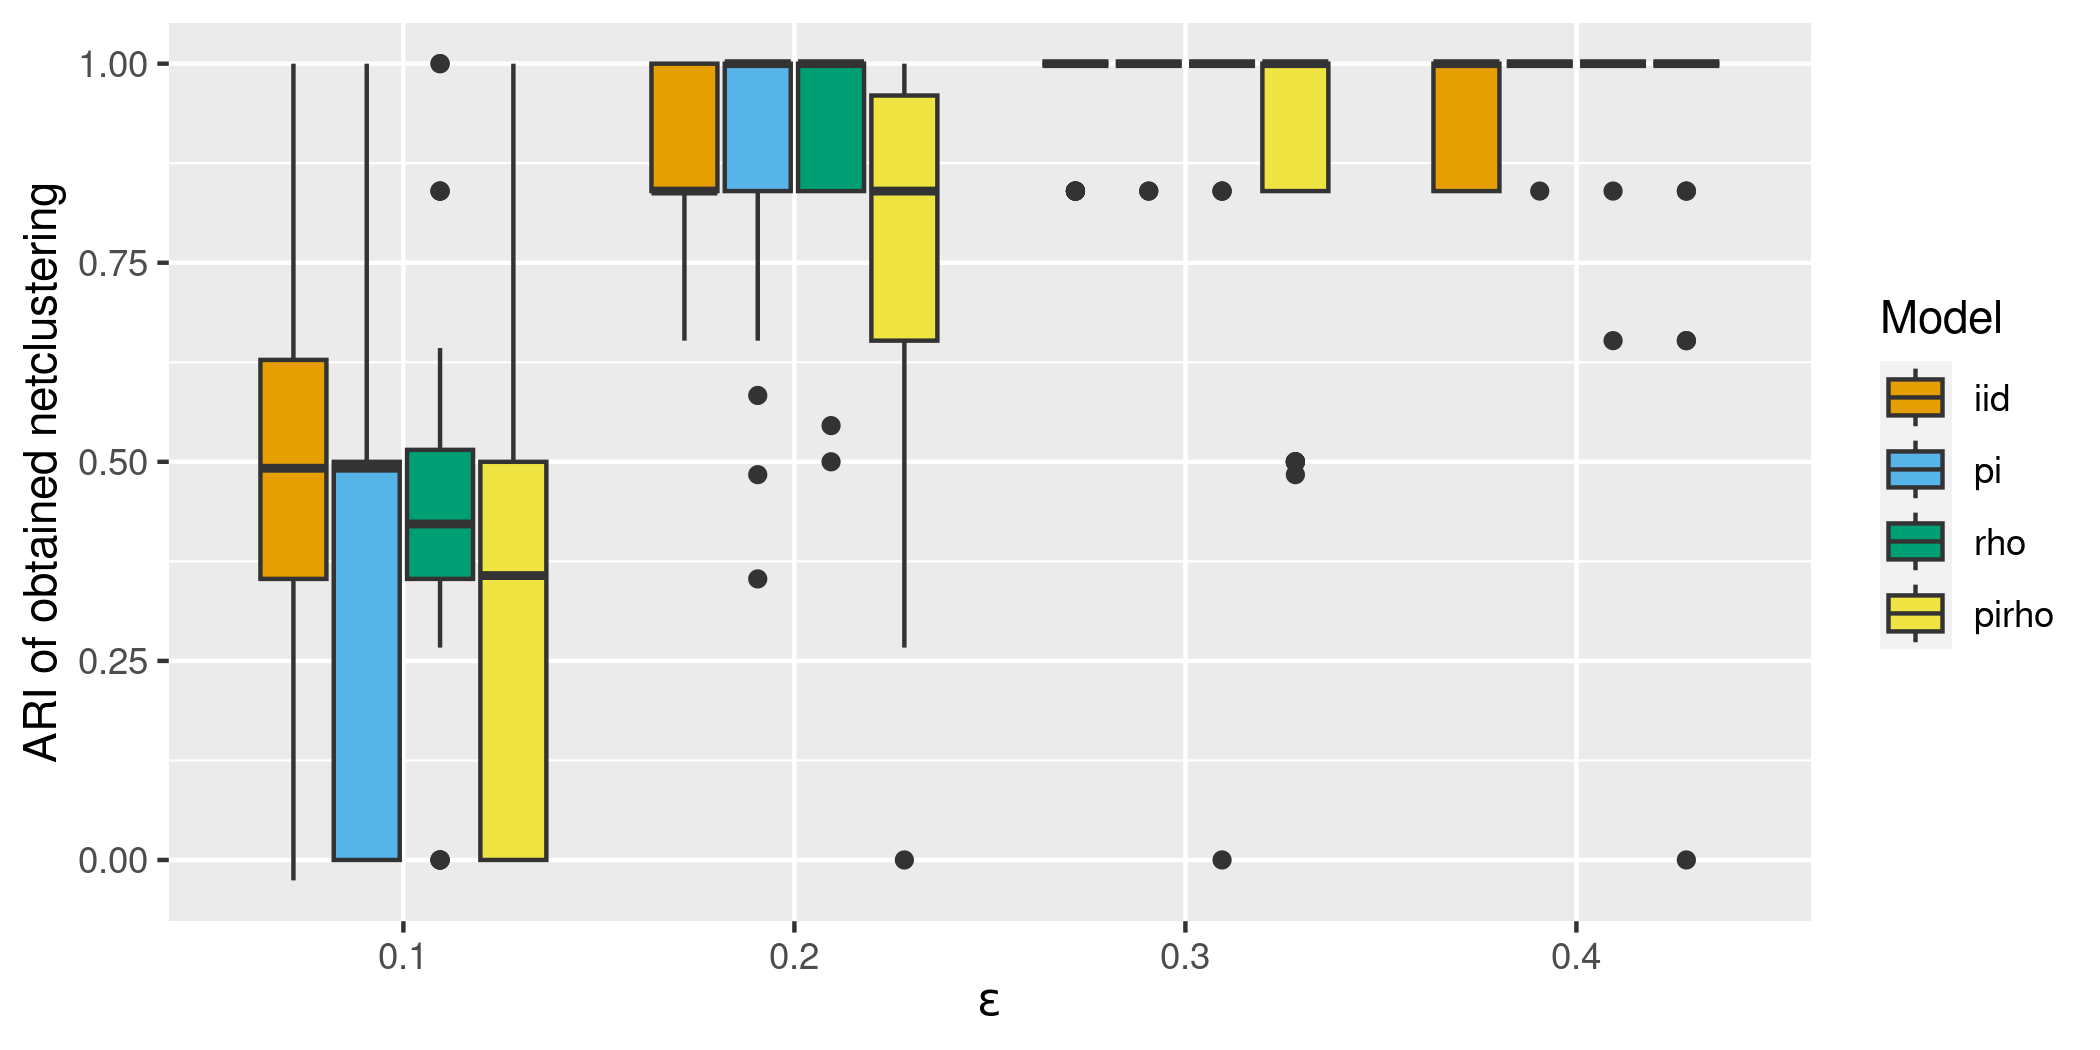
\includegraphics{./img/ca0adc96e26b9b41eb8dec4c472696309ebcf0fe.png}
\caption{\label{}ARI of the partition obtained by clustering in function
of \(\eps\)}
\end{figure}

\paragraph{Results}

The evaluation of our method involves a comparison between the resulting
partition of the network collection and the simulated partition using
the ARI index. As the value of \(\epsilon\) increases, our ability to
distinguish between the networks improves, and this distinction becomes
nearly perfect in all setups of the \(colBiSBM\).
